%%%%%     PACKS     %%%%%
\documentclass[12pt]{article}
\usepackage[margin=1in,headsep=.60in]{geometry}
\usepackage[utf8]{inputenc}
\usepackage[table, dvipsnames]{xcolor}
\usepackage{array}
\usepackage{amsmath}
\usepackage{booktabs}
\usepackage{mdframed} %For box around text
\usepackage{hyperref} %For hyperlinks in the PDF
\hypersetup{
    colorlinks=true,
    linkcolor=blue,
    filecolor=magenta,
    urlcolor=cyan,
}
\urlstyle{same}
\usepackage{amsthm}
\usepackage{amssymb}
\usepackage{amsfonts}
\usepackage{siunitx}
\usepackage{graphicx}
\usepackage{caption}
\usepackage{pgfplots}
\graphicspath{{Images/}}
\usepackage[colorinlistoftodos]{todonotes}
\usepackage{cleveref}
\usepackage[labelformat=simple]{subcaption}
\usepackage{grffile}
\usepackage{gensymb}
\usepackage{float}
\usepackage[shortlabels]{enumitem}
\usepackage{enumitem}
\setlistdepth{9}
\usepackage{biblatex} %Imports biblatex package
\addbibresource{references.bib}
\usepackage{outlines}
\usepackage{minted}
\usepackage{pdflscape}
\usepackage{everypage}
\usepackage{multirow}
\usepackage{multicol}
\usepackage{afterpage}
\usepackage[labelfont=bf, font=small]{caption}
\usepackage{upgreek}
\usepackage{tikz}
\usepackage{xcolor}
\usepackage{listings}

% style sheet for code
\definecolor{codegreen}{rgb}{0,0.6,0}
\definecolor{codegray}{rgb}{0.5,0.5,0.5}
\definecolor{codepurple}{rgb}{0.58,0,0.82}
\definecolor{backcolour}{rgb}{0.95,0.95,0.92}

\lstdefinestyle{mystyle}{
    backgroundcolor=\color{backcolour},   
    commentstyle=\color{codegreen},
    keywordstyle=\color{magenta},
    numberstyle=\tiny\color{codegray},
    stringstyle=\color{codepurple},
    basicstyle=\ttfamily\footnotesize,
    breakatwhitespace=false,         
    breaklines=true,                 
    captionpos=b,                    
    keepspaces=true,                 
    numbers=left,                    
    numbersep=5pt,                  
    showspaces=false,                
    showstringspaces=false,
    showtabs=false,                  
    tabsize=2
}

\lstset{style=mystyle}

\usepackage{lastpage}
%%%%%     COMMANDS     %%%%%
%%%% Blue box for subsection text (not figures) %%%%
\newenvironment{bluebox}
  {\begin{mdframed}[backgroundcolor=blue!5,linecolor=blue!40,roundcorner=8pt]}
  {\end{mdframed}}

%%%% Simple neutral box for figures %%%%
\newenvironment{figbox}
  {\begin{mdframed}[roundcorner=8pt,shadow=true,shadowsize=4pt,shadowcolor=black!40]}
  {\end{mdframed}}

\begin{document}

\begin{titlepage}
\newcommand{\HRule}{\rule{\linewidth}{0.5mm}}

\center

\textsc{\LARGE Aarhus University}\\[1.5cm]
\textsc{\Large Computer Science}\\[0.5cm]
\textsc{\large Numerical Linear Algebra}\\[0.5cm]
    

\HRule\\[0.4cm]
    \center 
    {\huge\bfseries Exam }\\[0.4cm] % Title of your document
\HRule\\[1.5cm]


\vfill\vfill\vfill % Position the date 3/4 down the remaining page
    
    {\large\today}

\vfill\vfill
    
\includegraphics[width=0.2\textwidth]{Aarhus_University_seal.png}\\[1cm] % Include a department/university logo - this will require the graphicx package
    

\vfill
\end{titlepage}
%%%%%      CHAPTERS      %%%%%
\hspace{0.02cm}
\section*{Problem 1}
Given the basis E:
\[
E:\; p_0(x) = 1 + x, \quad p_1(x) = 1- x, \quad p_2(x) = x + x^2 
\]
How many of each $p_i$ is needed to make $q(x) = 3 - 2x + x^2$, which is represented by a coordinate vector $[q]_E$.\\
This can also be explained by definition 19.6 and equation 19.1~\cite{NUMLA}
The answer is (B) $\begin{bmatrix}
    0 \\
    3 \\
    1
\end{bmatrix}$
which amounts to:
\[
0 (1+x) + 3(1-x) + x - x^2 = 3 - 2x + x^2 
\]
So $[q]_E = \begin{bmatrix}
    0 \\
    3 \\
    1
\end{bmatrix}
$
Answer (B)



\section*{Problem 2}
For $V = \mathbb{R}^{3\times 3}$ being the vector space for all real $3\times 3$ matrices.\\
it is given in the start of chapter 25 that for $A^T = A$ then $A$ is real symmetricthis means (B) hold as being in the subset of $V$\\
The answer is (B)

\section*{Problem 3}
\subsection*{(a)}
The shape can be determined by inserting an if statement for when $i = 3$\\
Note that the code is but a snippet, hence the import statement is ommited, and the final code is in the appendix, this will be the case for all code snippets.
\begin{lstlisting}[language=Python]
    def mgs(a):
    q = np.copy(a)
    r = np.zeros((8, 8))
    for i in range(8):
        r[i, i] = np.linalg.norm(q[:, i])
        q[:, i] /= r[i, i]
        r[[i], i+1:] = q[:, [i]].T @ q[:, i+1:]

        if(i == 3 ):
            print((q[:, [i]] @ r[[i], i+1:]).shape)

        q[:, i+1:] -= q[:, [i]] @ r[[i], i+1:]
    return q, r

u = np.ones((120,8))
mgs(u)
\end{lstlisting}
The output is $(120.8)$ which is the shape of $q[:, [i]] @ r[[i], i+1:]$ when $i = 3$

\subsection*{(b)}
The matrices are:
\[
(q[:,\; [3]].T)^{1 \times 120} \times (q[:,\; 3+1:])^{120 \times 4}
\]
so the resulting equation for calculating flops for matrix product is $2mkn = 2(1)(120)(4) = 960$\\
So the total amount of flaps used to compute the product is $960$ flops.\\
The formula for flops can be found in chapter 5 section 5.1~\cite{NUMLA}
\section*{Problem 4}
the most important note here is the relation between the eigenvalues for A
\[
-3, \quad 1, \quad 4, \quad 7.
\]
and S
\[
16, \quad 0, \quad 9, \quad 36.
\]
The pattern is each eigenvalue in A has been subtracted by one and multiplied by itself which results in all positive eigenvalues.\\
this means the answer can't be (B) $S(A^2-I_4)S^{-1}$ since it raises the power before subtracting with $I_4$.\\
If one uses theorem 7.2~\cite{NUMLA} then $SS^{-1} = I_4$ and in answer (C) $(SAS^{-1} - i_4)^2$ this becomes $(AI_4 -I_4)^2$ where each diagonal in $A$ is multiplied and subtracted by one before beign taken to the power of 2\\
In conclusion the answer is (C)


\section*{Problem 5}
Given the vectors
$w_0 =\begin{bmatrix}
    1 \\
    0 \\
    1 \\
    0
\end{bmatrix}$, $ w_1 =\begin{bmatrix}
    1 \\
    0 \\
    -1 \\
    0
\end{bmatrix}$ and $ w_2 = \begin{bmatrix}
    0 \\
    1 \\
    0 \\
    1
\end{bmatrix}$
\subsection*{(a)}
We form it's column matrix $W = [w_0 | w_1 | w_2]$
\[W =
\begin{bmatrix}
1.00 & 1.00 & 0.00 \\
0.00 & 0.00 & 1.00 \\
1.00 & -1.00 & 0.00 \\
0.00 & 0.00 & 1.00 \\
\end{bmatrix}
\]
then creating the gram-matrix from lemma 9.9~\cite{NUMLA}
\begin{lstlisting}
mat = np.array([[1,1,0],
                [0,0,1],
                [1,-1,0],
                [0,0,1]])
gram = mat.T @ mat
\end{lstlisting}
\[
G =
\begin{bmatrix}
2.00 & 0.00 & 0.00 \\
0.00 & 2.00 & 0.00 \\
0.00 & 0.00 & 2.00 \\
\end{bmatrix}
\]
Which according to lemma 9.9 if it's diagonal then it is orthogonal. and $G$ is diagonal since all entries except the diagonal is zero.\\
Hence the collection $w_0, w_1, w_2$ is orthogonal
\subsection*{(b)}


\section*{Problem 6}
\subsection*{(a)}
The system $Ax = y$ can be represented as
\[
\begin{bmatrix}
1.0 & 0.0 & \cos(0) \\
1.0 & 0.5 & \cos(0.5) \\
1.0 & 1.0 & \cos(1) \\
1.0 & 1.5 & \cos(1.5) \\
1.0 & 2.0 & \cos(2.0) \\
1.0 & 2.5 & \cos(2.5) \\
1.0 & 3.0 & \cos(3.0) \\
\end{bmatrix} \cdot \begin{bmatrix}
    a \\
    b \\
    c
\end{bmatrix}
= 
\begin{bmatrix}
    0.0 \\
    0.5 \\
    1.0\\
    1.5 \\
    2.0\\
    2.5 \\
    3.0\\
\end{bmatrix}
\]
The dimension of $A = 3\time 7$ and $x = 3\times 1$ and $y = 7\times 1$
\subsection*{(b)}
The function(s) used can be found in the appendix. It's a thin QR decompositon that uses the improve gram-schmidt and back substitution.
\begin{lstlisting}[language=Python]
c = np.cos
t = np.array([0.0, 0.5, 1.0, 1.5, 2.0, 2.5, 3.0])
y = np.array([3.05, 2.48, 1.62, 0.63, -0.17, -0.56, -0.48])

A = np.array([[1, t[0], c(t[0])],
              [1, t[1], c(t[1])],
              [1, t[2], c(t[2])],
              [1, t[3], c(t[3])],
              [1, t[4], c(t[4])],
              [1, t[5], c(t[5])],
              [1, t[6], c(t[6])]])
x_solution = solve_least_squares_qr(A, y)

print(x_solution)
    
\end{lstlisting}
The least-squared solution for the coefficients in $x$ are 
\[
\begin{bmatrix}
    1.4188\\
    -0.3553 \\
    1.3114
\end{bmatrix}
\]
Note that i've rounded the last decimal
\subsection*{(c)}
Using np.linspace and the function $f(t)$ with the coeeficients from (b), we fit it to the data points on the interval $0 \leq t \leq 3$\\
The code is a continuation of the previosu snippet from (b)
\begin{lstlisting}[language = Python]
t_interval = np.linspace(0, 3 , 500)

yy_interval = x_solution[0,0]  + x_solution[1,0]*t_interval + x_solution[2,0]*c(t_interval) 

plt.figure(figsize=(9, 5))
plt.plot(t, y, 'o', color='black', label='Data points')
plt.plot(t_interval, yy_interval, '-', color='blue', label=f'fitted data')
plt.xlabel('$t$')
plt.ylabel('$y$')
plt.title(f'Problem 6: data point and fitted function f(t), interval 0 to 3 for t')
plt.grid(True, linestyle=':', alpha=0.6)
plt.legend()
plt.show()
\end{lstlisting}
\begin{figure}[H]
    \centering
    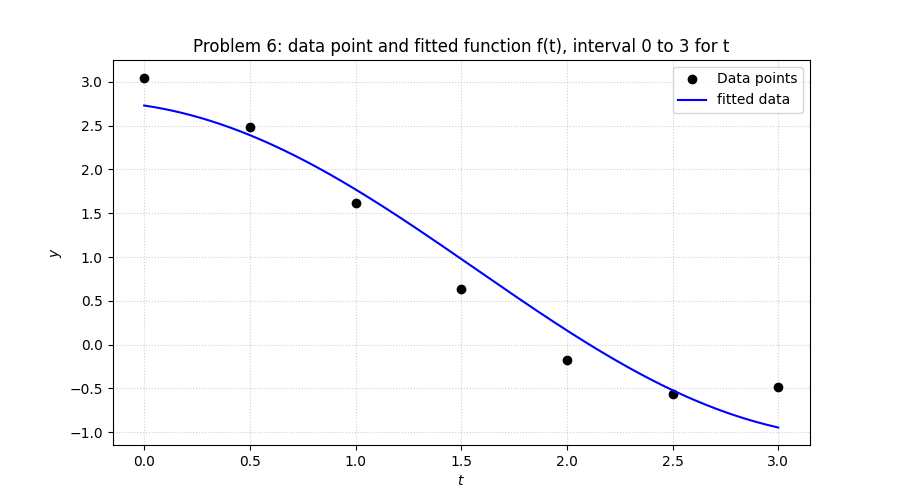
\includegraphics[width=0.8\textwidth]{problem6c.png}
\end{figure}
\subsection*{(d)}
From chapter 16.1~\cite{NUMLA} the residual vector is described aswell as the norm.\\
The residual vector is $r = b - Ax$:
\[r =
\begin{bmatrix} 
    0.3198 \\
    0.0880 \\
    -0,1520 \\
    -0.3486 \\
    -0.3324 \\
    -0.0399\\
    0.4653
\end{bmatrix}
\]
and it's norm
\[
||r||_2 =
0.7637
\]
The following is the code used for this\\
Again, a continuation of the previous snippet.
\begin{lstlisting}[language=Python]
yy_true = x_solution[0,0]  + x_solution[1,0]*t + x_solution[2,0]*c(t) 

residual = y - yy_true
residual_norm = np.linalg.norm(residual) 
deviation = np.abs(y - yy_true)
    
max_idt = np.argmax(deviation)
t_max_fail = t_interval[max_idt]
max_fail_val = deviation[max_idt]
   
\end{lstlisting}
The biggest deviation in the interval [0, 3] are 0.4653 and found with t = 0.0361\\
Which is the essentially the starting point.
\section*{Problem 7}

\section*{Appendix}
\begin{lstlisting}[language=Python, caption=Example Python code]
import numpy as np
import matplotlib.pyplot as plt
import sympy as sp

def back_subs(r, c):
    _, n = r.shape
    x = np.empty((n, 1))
    for i in reversed(range(n)):
        x[i] = (c[i] - r[[i], i+1:] @ x[i+1:]) / r[i, i]
return x


def forbedret_gram_schmidt(A):
   
    _, n = A.shape
    Q = A.copy().astype(float)
    R = np.zeros((n, n))
    for i in range(n):
        R[i, i] = np.linalg.norm(Q[:, i])
        Q[:, i] /= R[i, i]
        for j in range(i + 1, n):
            R[i, j] = np.vdot(Q[:, i], Q[:, j])
            Q[:, j] -= R[i, j] * Q[:, i]
    return Q, R

def solve_least_squares_qr(A, b):
    Q, R = forbedret_gram_schmidt(A)
    c = Q.T @ b
    return back_subs(R, c)


## Problem 3 code
def mgs(a):
    q = np.copy(a)
    r = np.zeros((8, 8))
    for i in range(8):
        r[i, i] = np.linalg.norm(q[:, i])
        q[:, i] /= r[i, i]
        r[[i], i+1:] = q[:, [i]].T @ q[:, i+1:]

        if(i == 3 ):
            print((q[:, [i]] @ r[[i], i+1:]).shape)

        q[:, i+1:] -= q[:, [i]] @ r[[i], i+1:]
    return q, r

u = np.ones((120,8))
mgs(u)
##############


### Problem 5 code
mat = np.array([[1,1,0],
                [0,0,1],
                [1,-1,0],
                [0,0,1]])
gram = mat.T @ mat


### Problem 6 code
c = np.cos
t = np.array([0.0, 0.5, 1.0, 1.5, 2.0, 2.5, 3.0])
y = np.array([3.05, 2.48, 1.62, 0.63, -0.17, -0.56, -0.48])

A = np.array([[1, t[0], c(t[0])],
              [1, t[1], c(t[1])],
              [1, t[2], c(t[2])],
              [1, t[3], c(t[3])],
              [1, t[4], c(t[4])],
              [1, t[5], c(t[5])],
              [1, t[6], c(t[6])]])
x_solution = solve_least_squares_qr(A, y)

print(x_solution)

t_interval = np.linspace(0, 3 , 500)

yy_interval = x_solution[0,0]  + x_solution[1,0]*t_interval + x_solution[2,0]*c(t_interval) 

plt.figure(figsize=(9, 5))
plt.plot(t, y, 'o', color='black', label='Data points')
plt.plot(t_interval, yy_interval, '-', color='blue', label=f'fitted data')
plt.xlabel('$t$')
plt.ylabel('$y$')
plt.title(f'Problem 6: data point and fitted function f(t), interval 0 to 3 for t')
plt.grid(True, linestyle=':', alpha=0.6)
plt.legend()
plt.show()


yy_true = x_solution[0,0]  + x_solution[1,0]*t + x_solution[2,0]*c(t) 

residual = y - yy_true
residual_norm = np.linalg.norm(residual) 
deviation = np.abs(y - yy_true)
    
max_idt = np.argmax(deviation)
t_max_fail = t_interval[max_idt]
max_fail_val = deviation[max_idt]
   


\end{lstlisting}
    


\printbibliography



\end{document}y